\documentclass[xcolor=pdftex,dvipsnames,table,mathserif,aspectratio=169]{beamer}
\usetheme{metropolis}
%\usetheme{Darmstadt}
%\usepackage{times}
%\usefonttheme{structurebold}

\usepackage[english]{babel}
%\usepackage[table]{xcolor}
\usepackage{pgf,pgfarrows,pgfnodes,pgfautomata,pgfheaps}
\usepackage{amsmath,amssymb,setspace}
\usepackage[latin1]{inputenc}
\usepackage[T1]{fontenc}
\usepackage{relsize}
\usepackage[absolute,overlay]{textpos} 
\newenvironment{reference}[2]{% 
  \begin{textblock*}{\textwidth}(#1,#2) 
      \footnotesize\it\bgroup\color{red!50!black}}{\egroup\end{textblock*}} 

\DeclareMathSizes{10}{10}{6}{6} 


\title [``Old'' IO]{Before there was ``New'' Empirical IO}
\author{C.Conlon}
\institute{Grad IO }
\date{Fall 2019}
\setbeamerfont{equation}{size=\tiny}
\begin{document}

\begin{frame}
\titlepage
\end{frame}

\begin{frame}{Early Stuff}
This lecture is a bit different from all of the others
\begin{itemize}
\item Focus is primarily on theory rather than empirics
\item History of approaches (some of which have fallen out of fashion).
\item Should be familiar to most of you
\begin{itemize}
\item Brush up on first few chapters of Tirole (1988) (somewhat dated) but still the best reference for oligopoly theory.
\item Vives (2000) is a more modern (and focused) review of oligopoly theory.
\item I assume familiarity with an undergrad text like Carlton and Perloff (1999), Cabral (2000) or Shy (1996).
\end{itemize}
\end{itemize}
\end{frame}


\begin{frame}{History of IO: Part I}
Structure-Conduct-Performance (1940-1960) Harvard
\begin{itemize}
\item Associated with the work of Joe Bain.
\item Structure (number of firms, market shares, etc.). Barriers to entry are key.
\item Structure $\rightarrow$ conduct (ie: how firms behave)
\item Conduct $\rightarrow$ performance (ie: prices, markups, efficiency)
\item Use accounting data to get performance (profits, price-cost margins, etc.)
\item OLS regression across industries to see whether profits are higher in more concentrated industries.
\item Empirics were somewhat atheoretic.
\end{itemize}
Complaint: the direction of causality is assumed. (Don't profits determine number of entrants too?).
\end{frame}

\begin{frame}{History of IO: Part II}
Chicago School (1960-1980)
\begin{itemize}
\item Most associated with the work of George Stigler and later Robert Bork ``Antitrust Paradox''
\item Monopoly is more often alleged than confirmed
\item Even when monopoly does exist -often only temporary (did MSFT take over the world?)
\item Entry and threat of entry is crucial.
\item Emphasis on price theory (markets work) and better econometrics
\item Still quite persuasive for practice of anti-trust (judges and lawyers).
\end{itemize}
\end{frame}


\begin{frame}{History of IO: Part III}
Game Theory (1980-1990s)
\begin{itemize}
\item For most of the 1980s, IO was dominated by game theorists.
\item Strategic decision making, Nash Equilibrium
\item Lots of intuitive (and sometimes counter-intuitive) clean theoretical models
\item Hard to know which model is the right model for the industry we are looking at.
\end{itemize}
\end{frame}


\begin{frame}{History of IO: Part IV}
The not so ``new'' anymore empirical IO (NEIO) (1989-)
\begin{itemize}
\item Back to one industry at a time.
\item Careful game-theoretical model of industry behavior
\item Joined with modern econometrics, data, and computation.
\end{itemize}
\end{frame}


\begin{frame}{The Monopoly Problem}
Start with a quantity-setting monopolist facing a known inverse demand curve $P(Q)$ and costs $C(Q)$.
\begin{eqnarray*}
\pi(Q) = P(Q) \cdot Q - C(Q) -  F
\end{eqnarray*}
Take the FOC:
\begin{eqnarray*}
\pi'(Q) &=& 0  \\
 \underbrace{\overbrace{P'(Q) \cdot Q}^{\text{\alert{monopoly distortion}}}+ P(Q)}_{MR}  &=&  \underbrace{C'(Q)}_{MC} \\
  \frac{P(Q) - C'(Q)}{P(Q)} &=& - \frac{P'(Q) \cdot Q}{P(Q)} = \frac{1}{|\epsilon_d|}
\end{eqnarray*}
\begin{itemize}
\item This is known as the \textit{Lerner (1934) Index} or \alert{economic markup}.
\end{itemize}
\end{frame}

\begin{frame}{The Monopoly Problem}
We could have rewritten it as 
\begin{eqnarray*}
P \left( 1+\frac{1}{\epsilon_d} \right) = MC
\end{eqnarray*}
\begin{itemize}
\item This is helpful because it shows us the important result that the monopolist never produces in the inelastic portion of the demand curve. $\epsilon_d \in (-1,0]$.
\item Why? MR is negative! Reduce Quantity!
\item Often data report: $\frac{P-MC}{MC}= \frac{1}{\epsilon_d -1}$. But we usually work with the Lerner formula in IO.
\item For the monopolist firm level elasticity $\epsilon_d$ is the same as $\epsilon_D$ the market elasticity.
\end{itemize}
\end{frame}


\begin{frame}{Cournot Model (1838) / Nash in Quantities}
\begin{itemize}
\item I am going to assume constant marginal cost $c_i = c$ and $n$ equal sized firms to make life easy. 
\item We let $Q=\sum_{i=1}^N q_i$ the total output of the industry.
\end{itemize}
We consider profits and FOC's:
\begin{eqnarray*}
\pi_i(q_i) &=& (P(Q) - C_i'(q_i) ) \cdot q_i\\
\frac{\partial \pi_i(q_i)}{\partial q_i} &=& (P(Q) - C_i'(q_i))  +  q_i  \cdot P'(Q) \cdot \frac{\partial Q}{\partial q_i}  = 0
\end{eqnarray*}
Cournot competition implies that $\frac{\partial Q}{\partial q_i} = 1$ and $\frac{\partial q_j}{\partial q_i} = 0$ for $i \neq j$ (this is because it is a simultaneous move game).
\begin{eqnarray*}
P(Q) + P'(Q) \cdot q_i = \underbrace{P(Q) + \overbrace{P'(Q) \cdot \frac{Q}{n}}}^{\text{\alert{Cournot Distortion}}}_{MR} =  mc
\end{eqnarray*}
\end{frame}

\begin{frame}{Cournot Model (1838) / Nash in Quantities}
Rearrange to form the Lerner Index:
\begin{eqnarray*}
\frac{P-mc}{P} = - \frac{1}{n} \frac{Q}{P} P'(Q) = - \frac{1}{n \cdot \epsilon_D}
\end{eqnarray*}
Some notes
\begin{itemize}
\item In general market demand is much less elastic than firm level demand.
\item When things are symmetric then we can relate aggregate to firm level elasticity: $\epsilon_d = n \cdot \epsilon_D$.
\item For beer market demand $\epsilon_D \approx -0.8$. If $n=5$ then a typical firm faces an elasticity of $-4.0$.
\item We can back out implied markups pretty easily: $P  = \frac{MC}{1-(1/\epsilon_d)}  = \frac{4}{3} MC$.
\item Market demand can be at inelastic part of curve -- but firm level demand cannot.
\end{itemize}
\end{frame}


\begin{frame}{Betrand Paradox (1883)/ Nash in Prices}
Briefly contrast with Bertrand
\begin{itemize}
\item Two firms with symmetric marginal costs $c_i=c$.
\item Nash in prices means that $p = c$.
\item This is not very interesting or helpful.  Also firms make profits!
\item Solutions

\begin{itemize}
\item Add capacity constraints (starts to behave like Cournot again (Kreps Scheinkman)).
\item Add other frictions (search costs?)
\item Add product differentiation (mostly we focus on this).
\end{itemize}
\end{itemize}
\end{frame}


\begin{frame}{Asymmetric Cournot and HHI}
\begin{itemize}
\item Symmetry doesn't seem like a particularly realistic assumption.
\item We can extend this to the asymmetric case pretty easily by modifying the \alert{Cournot distortion}: $q_i \cdot P'(Q) \cdot \frac{\partial Q}{\partial q_i}$.
\item Instead we have that $\frac{q_i}{Q} \cdot \frac{\partial Q}{\partial q_i} = \frac{q_i}{\sum_{j=1}^n q_j} \equiv s_i$ or \alert{market share}.
\item Obviously this nests symmetric case where $q_i = \frac{Q}{n}$ or $s_i = \frac{1}{n}$.
\item The Cournot markup / Lerner Index is just
\begin{eqnarray*}
\frac{P-mc_i}{P} = \frac{s_i}{|\epsilon_D|}
\end{eqnarray*}
\item Cournot: markups are proportional to market-share.
\item Nests perfect competition $n \rightarrow \infty$ or $s_i \rightarrow 0$.
\item Semi-joke: IO economists say something is \alert{intuitive} if it follows Cournot predictions.
\end{itemize}
\end{frame}


\begin{frame}{Asymmetric Cournot and HHI}
Now consider the market share weighted Lerner index:
\begin{eqnarray*}
HHI = \sum_{i=1}^N \frac{P - mc_i}{P} s_i = \sum_{i=1}^n \frac{s_i^2}{\epsilon_D}
\end{eqnarray*}
\begin{itemize}
\item For $\epsilon_D =1$, this is known as the \alert{Hirschman-Herfindal Index}.
\item This gives us a measure of \alert{market concentration} that varies from 0 to 10,000 (units of $s_i$ are in percentages).
\item DOJ/FTC describe markets as:
\begin{itemize}
\item Highly Concentrated: $HHI \geq 2500$.
\item Moderately Concentrated: $HHI \in [1500,2500]$. $\Delta HHI \geq 250$ merits scrutiny.
\item Un-Concentrated: $HHI \leq 1500$.
\end{itemize}
\end{itemize}
\end{frame}

\begin{frame}{Asymmetric Cournot and HHI}
\begin{itemize}
\item Can also work backwards form HHI to get effective ``number of firms''.
\item Here HHI is in units of $[0,1]$ instead of $[0,10000]$.
\begin{eqnarray*}
HHI = \sum_{i=1}^N s_i^2 = \frac{1}{n^*} \rightarrow n^{*} = \frac{1}{HHI}.
\end{eqnarray*}
\item ex. Four firms with shares $40\%, 30\%, 15\%, 15\%$. So the $HHI =.295$. Thus $n^{*} = 1/.295 = 3.39$ and $\epsilon_d = \epsilon_D \cdot 3.39$.
\item Alternatively (under Cournot only!) can write:
\begin{eqnarray*}
\frac{P-MC}{P} = \frac{HHI}{\epsilon_D}
\end{eqnarray*}

\end{itemize}
\end{frame}

\begin{frame}{Alternatives to HHI}
\begin{itemize}
\item Another alternative is the $k$ firm concentration ratio $CR_k = \sum_{i=1}^N s_i$.
\item This can be useful as an additional descriptive statistic.
\item It shows up in some older work
\item $4$ firms is a popular measure.
\end{itemize}
\end{frame}


\begin{frame}{Complaints about HHI}
\begin{itemize}
\item HHI only measures market power under the Cournot assumptions
\begin{itemize}
\item Holding competitor's output responses fixed so that $\frac{\partial Q}{\partial q_i} =1$.
\item Competition is about setting quantity rather than price: strong restrictions on cross-price elasticities.
\item Is quantity (instead of price) the relevant strategic variable? (Sometimes...).
\end{itemize}
\item Assumes that products are \alert{homogenous} so that all firms/products are equally good competitors.
\item More concentrated markets have higher markups, but not always lower welfare (allocating production from low to high cost firms might improve welfare).
\end{itemize}
\end{frame}

\begin{frame}{Conjectural Variations}
\begin{itemize}
\item If I change my quantity, why doesn't my rival?
\item Biggest complaint about Cournot is that we hold quantities of competitors fixed
\item Suppose we did not so that $\frac{\partial Q_i}{\partial q_i} = (1 + \frac{\partial Q_{-i}}{\partial q_i}).$
\item FOC becomes:
\begin{eqnarray*}
P + P'(Q) \cdot q_i \cdot \underbrace{\left(1+ \frac{\partial Q_{-i}}{\partial q_i} \right)}_{\theta_i}
\end{eqnarray*}
\item $\frac{\partial Q_{-i}}{\partial q_i} =-1$  or $\theta_i =0$ corresponds to competition (aggregate quantity is unchanged). (also Bertrand)
\item $\frac{\partial Q_{-i}}{\partial q_i} =0$ or $\theta_i = 1$ corresponds to the Cournot model.
\item $\frac{\partial Q_{-i}}{\partial q_i} =N-1$ or $\theta_i = N$ corresponds to the joint profit maximization (collusion/monopoly).
\item This was great for applied theory, now I can nest all of the key classical models (PC, monopoly, Cournot) with a single parameter.
\end{itemize}
\end{frame}

\begin{frame}{Conjectural Variations: Issues}
\begin{itemize}
\item On one hand seems like more flexibility was a good thing.
\item On the other hand with some $\theta_i$ we can justify nearly anything.
\item Two questions
\begin{enumerate}
\item Can we expect to recover $\theta_i$ from data?
\item What about \alert{consistent conjectures} (ie: suppose I require firms to actually want to respond in the way that I believe they will).
\end{enumerate}
\end{itemize}
\end{frame}



\begin{frame}{Consistent Conjectures}
\begin{itemize}
\item Bresnahan (1981) posed the consistent conjectures hypothesis (one unique conjecture that satisfied all FOCs simultaneously).
\item Large theory literature that followed [see Daughety (1985) or Lind(1992)] show Cournot $\theta_i=0$ is the only consistent conjecture absent some knife-edge cases.
\item This basically meant that CV approaches fell out of favor with game theorists by the late 1980s/early 1990s.
\item Things are even more problematic for dynamic models.
\item The approach persisted in empirical work until Corts (1999) [more on this later].
\end{itemize}
\end{frame}

\begin{frame}{Can/Should we try and recover $\theta_i$ from data?}
\begin{figure}
\begin{center}
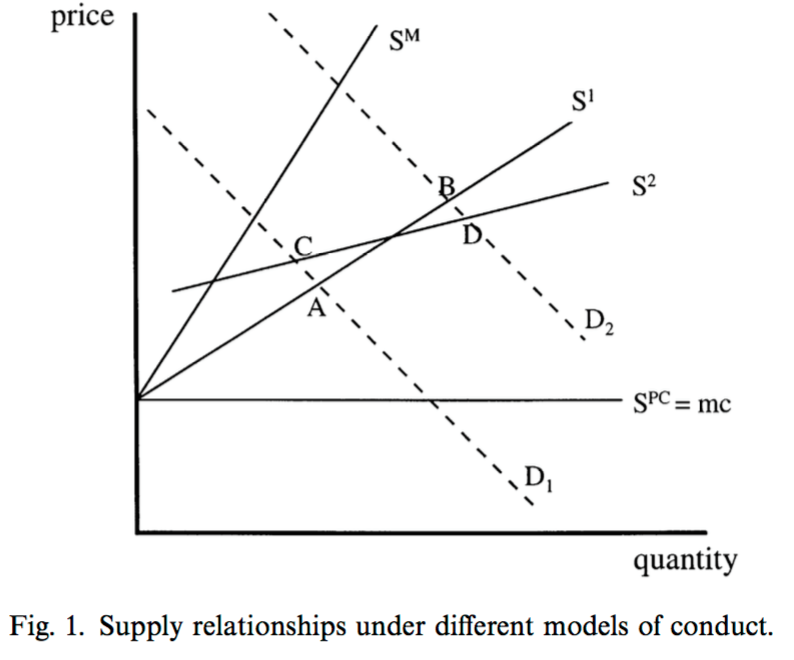
\includegraphics[width=4in]{resources/cortsfigure.png}
\end{center}
\end{figure}
\end{frame}



\begin{frame}{Testing S-C-P }
Can we test for relationship between performance and market structure?
\begin{itemize}
\item Positive correlation between $HHI$ and market power.
\begin{itemize}
\item Usually easy to measure concentration (sort of)
\item Measuring Profits is tough:
\begin{itemize}
\item Accounting profits: taxes and depreciation aren't really very close $P-MC$.
\item Tobin's Q
\item The Lerner index: $(P-MC)/P$
\end{itemize}
\item We don't usually get to observe $MC$ in data.

\begin{itemize}
\item Maybe we see something like total revenue or total variable cost and units sold.
\item Have to use unit values $(P-AVC)/P$ which is okay if $AVC \approx MC$ and our firm sells only a single product at a single $P$.
\item Trade data sometimes looks a bit like this today...
\end{itemize}
\end{itemize}
\end{itemize}
\end{frame}


\begin{frame}{S-C-P paradigm and empirical work}
Bain (1951)
\begin{itemize}
\item Census data was across industries but not firm-level data.
\item Prices are hard to compare across industries (for obvious reasons)
\item Profits/Markups are easier to measure and compare across industries
\item Firms make profits was an important stylized fact at the time.
\end{itemize}
Why do we care?
\begin{itemize}
\item The whole basis for modern antitrust and regulation is based on the relationship between concentration and market power.
\end{itemize}
\end{frame}

\begin{frame}{S-C-P regressions \#1}
\begin{eqnarray*}
y = \beta_0 + \beta_1 \cdot HHI + \gamma X +  \varepsilon
\end{eqnarray*}

\begin{itemize}
\item Using $y$ as profit measure and each observation a different industry.
\item Idea is that $\beta_1 > 0$ meant increased concentration meant higher profits (or prices).
\item Lots of different $X$'s (controlling for returns to scale, R\&D, etc.): anything that shifts profits that isn't competition.
\item We should probably worry that $E[\varepsilon | H, X ] = 0$ or that factors might be correlated with both profitability and concentration in unobservable ways.
\begin{itemize}
\item Is Google or Facebook or Apple highly profitable because of concentration?
\end{itemize}
\item Structure, Prices, and Profits are likely simultaneously determined.
\end{itemize}
\end{frame}

\begin{frame}{S-C-P regressions \#2}
\begin{eqnarray*}
y_{if} = \beta_0 + \beta_1 \cdot HHI_i + \beta_2 s_{if} +  \gamma X_{i} +  \varepsilon
\end{eqnarray*}
\begin{itemize}
\item One critique (associated with Demsetz (1973) and the Chicago School) was the following
\begin{itemize}
\item With firm level data if we include share of the firm $s_{if}$ the coefficient on that $\beta_2$ was positive and significant but any effect on $\beta_1$ became insignificant.
\item Even when it looked like concentration led to high prices, it meant that share was correlated with high prices
\item Chicago School took this as vindication of idea that larger firms were more efficient, had lower costs, etc.
\item Of course this is also what would be predicted from a standard Cournot model...
\end{itemize}
\end{itemize}
\end{frame}


\begin{frame}{S-C-P: Schmalensee 1989}
A huge handbook chapter summarizing the early literature that collected stylized facts.
\footnotesize
\begin{itemize}
\item Correlations among accounting profit measures are high but correlations between accounting measures and price-cost margins are low and results depend on which type of measure is used.
\item Cross industry accounting rates of return are too low to reconcile with standard monopoly models.
\item Accounting profitability differences among large firms are highly persistent
\item Industry characteristics account for only 10-25\% of cross sectional variation in accounting rates of return
\item Recent revenue growth is positively correlated with profitability
\item Relation between profitability and concentration is weak and effect is usually small. This relationship is not stable over item or industry and disappears with various controls.
\item Measures of scale economies or capital requirements are positively correlation with industry-level accounting profits
\item R\&D is positively related to profits but effect varies with $HHI$.
\item Profitability of largest firms is correlated with industry $HHI$ not true for smaller firms.
\end{itemize}
\end{frame}

\begin{frame}{S-C-P: What Happened?}

\begin{itemize}
\item Hundreds of papers written looking at correlations between $HHI$ and $\pi$ or $PCM$.
\item This literature has been dead for a while.
\begin{itemize}
\item We moved on from descriptive correlations to causes.
\item We generally need more of a theory to ascertain causes.
\item Data on individual industries and firms has gotten much better over time.
\end{itemize}
\item There are still lots of papers that try and infer causality from regressions like 
\begin{eqnarray*}
\pi_{it} = \alpha + \gamma HHI_{it} + \beta X_{it} + \epsilon_{it} 
\end{eqnarray*}
\item Mostly they will get rejected from journals if an IO economist sees it.
\item Market structure is \alert{endogenous} and there is no instrument for $HHI$.
\item Supply and demand are determined \alert{simultaneously} (so real problem is worse).
\end{itemize}
\end{frame}



\end{document}













































